%Document setup and layout
\documentclass[a4paper]{article}
\usepackage[utf8]{inputenc}
\usepackage[spanish]{babel}
\usepackage[T1]{fontenc}
\usepackage{listingsutf8}
\usepackage{makeidx}

%Images and figures
\usepackage{graphicx}
\usepackage{subcaption}
\usepackage[justification=centering]{caption}
\usepackage{float}

%Extras
\usepackage{underscore}
\usepackage{url}
\usepackage{color}
\usepackage{todonotes}
\usepackage[colorlinks=false]{hyperref}
\usepackage{fancybox}
\usepackage{tkz-graph}
\usetikzlibrary{arrows,positioning,automata}
%Tablas lindas
\usepackage{tikz}    
\usetikzlibrary{shadows}

%%%%%%%%%%%%%%%%%%%%%%%%%%%%%%%%%%%%%%%%%%%%%%%%%%%
%Para insertar dos imágenes, una al lado de la otra
%\begin{figure}[H]
%\centering
%\begin{minipage}{.5\textwidth}
%  \centering
%  \includegraphics[width=\linewidth]{path/a/imagen1}
%  \captionof{figure}{caption img 1}
%\end{minipage}%
%\begin{minipage}{.5\textwidth}
%  \centering
%  \includegraphics[width=\linewidth]{path/a/imagen2}
%  \captionof{figure}{caption img 2}
%\end{minipage}
%\end{figure}
%%%%%%%%%%%%%%%%%%%%%%%%%%%%%%%%%%%%%%%%%%%%%%%%%%%

\begin{document}

\section*{Informe}

En este informe se detallan los resultados del ejercicio 3 de la práctica de bordes y esquinas. Utilizamos la imagen de Lena y la de test para estos experimentos, pero mostramos sólo la de Lena para no extendernos demasiado.

\begin{figure}[H]
\centering
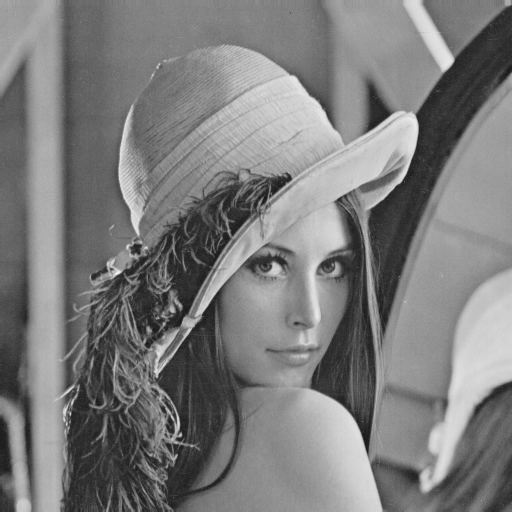
\includegraphics[width=0.25\textwidth]{imagenesInforme/lena}
\caption{Imagen original de Lena}
\end{figure}

\subsection*{Non-maximum supression}

\begin{figure}[H]
\centering
	\begin{subfigure}[t]{0.3\textwidth}
	\centering
	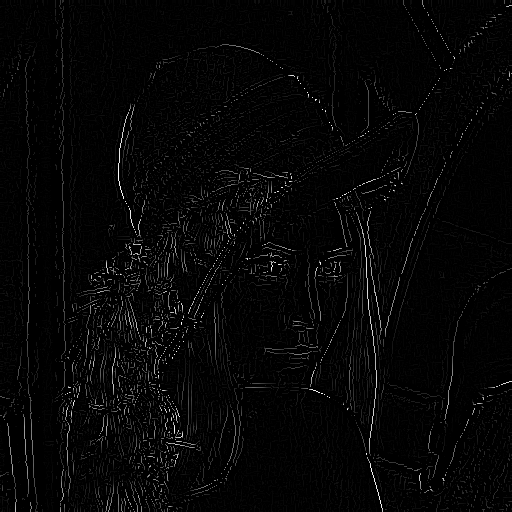
\includegraphics[width=\textwidth]{imagenesInforme/lenaNonMaximumSupressionSobel}
	\caption{Sobel}
	\end{subfigure}
	\begin{subfigure}[t]{0.3\textwidth}
	\centering
	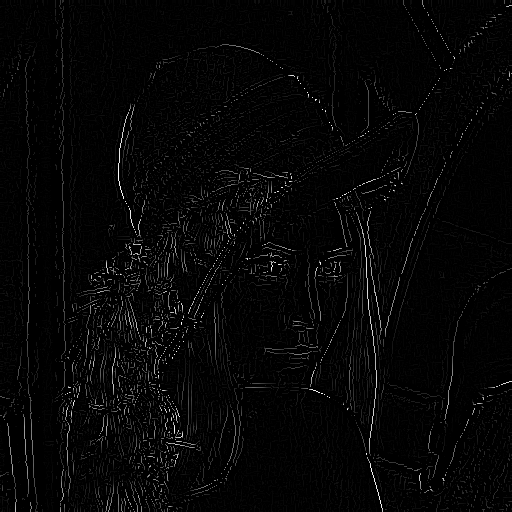
\includegraphics[width=\textwidth]{imagenesInforme/lenaNonMaximumSupressionPrewitt}
	\caption{Prewitt}
	\end{subfigure}
	\begin{subfigure}[t]{0.3\textwidth}
	\centering
	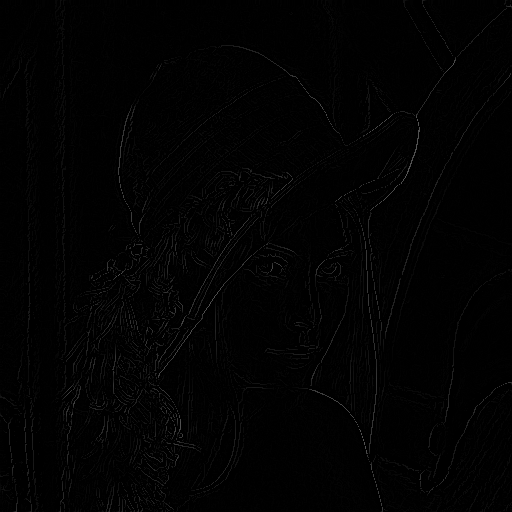
\includegraphics[width=\textwidth]{imagenesInforme/lenaNonMaximumSupressionRoberts}
	\caption{Roberts}
	\end{subfigure}
\caption{Con non-maximum supression}
\end{figure}

Podemos observar que aún sin histéresis, se notan bien los bordes de la imagen para cada método. Roberts no marca tan fuertemente los bordes, así que tal vez debería aplicársele histéresis. 

En las siguientes figuras se muestran las imágenes con non-maximum supression contaminadas con distintos tipos de ruidos, comenzando con el gaussiano.

\begin{figure}[H]
\centering
	\begin{subfigure}[t]{0.3\textwidth}
	\centering
	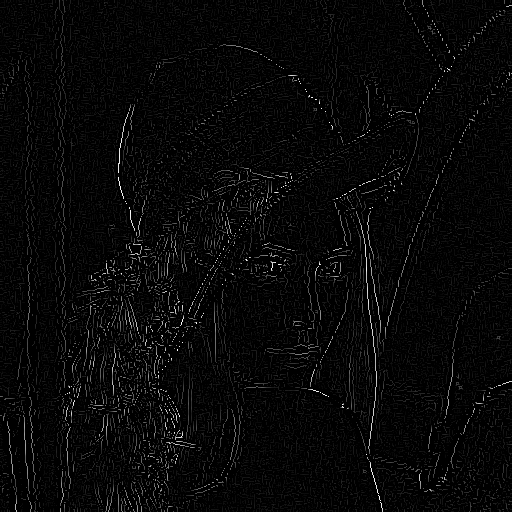
\includegraphics[width=\textwidth]{imagenesInforme/lenaNonMaximumSupressionGaussianSobel}
	\caption{Sobel}
	\end{subfigure}
	\begin{subfigure}[t]{0.3\textwidth}
	\centering
	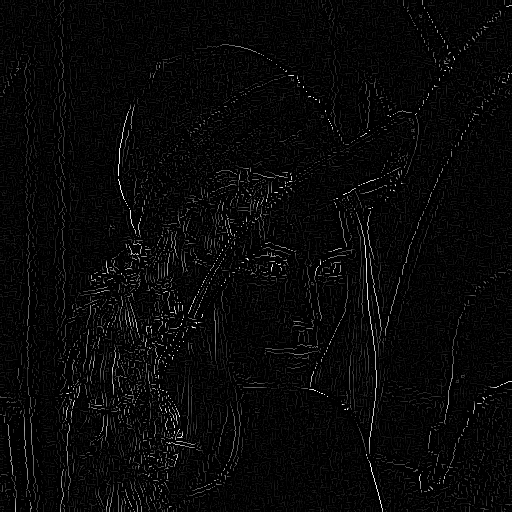
\includegraphics[width=\textwidth]{imagenesInforme/lenaNonMaximumSupressionGaussianPrewitt}
	\caption{Prewitt}
	\end{subfigure}
	\begin{subfigure}[t]{0.3\textwidth}
	\centering
	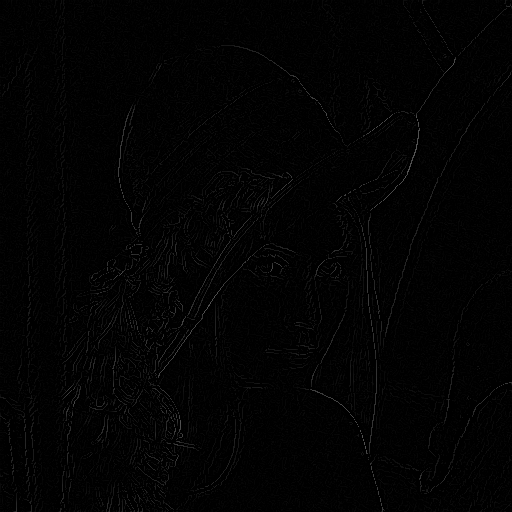
\includegraphics[width=\textwidth]{imagenesInforme/lenaNonMaximumSupressionGaussianRoberts}
	\caption{Roberts}
	\end{subfigure}
\caption{Con ruido gaussiano aditivo y non-maximum supression}
\end{figure}

Pareciera ser que la introducción de poco ruido aditivo gaussiano no cambia mucho el resultado. Aunque tal vez remarcar los bordes más fuertemente mostraría que se introdujo este ruido.

\begin{figure}[H]
\centering
	\begin{subfigure}[t]{0.3\textwidth}
	\centering
	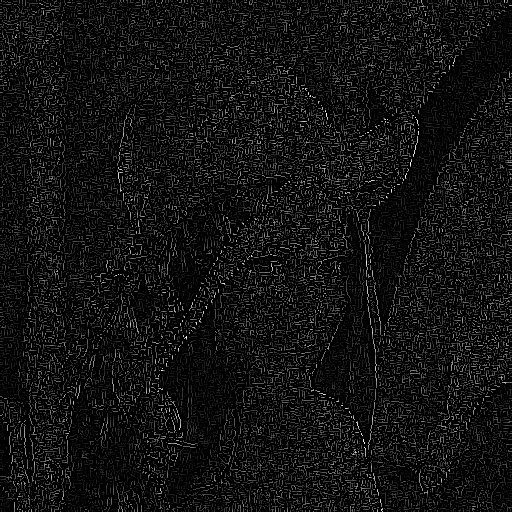
\includegraphics[width=\textwidth]{imagenesInforme/lenaNonMaximumSupressionRayleighSobel}
	\caption{Sobel}
	\end{subfigure}
	\begin{subfigure}[t]{0.3\textwidth}
	\centering
	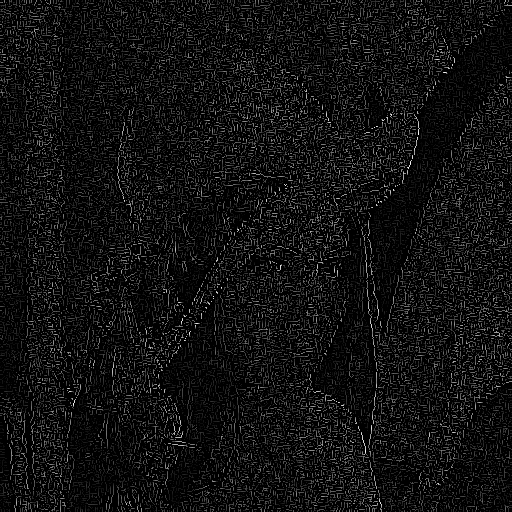
\includegraphics[width=\textwidth]{imagenesInforme/lenaNonMaximumSupressionRayleighPrewitt}
	\caption{Prewitt}
	\end{subfigure}
	\begin{subfigure}[t]{0.3\textwidth}
	\centering
	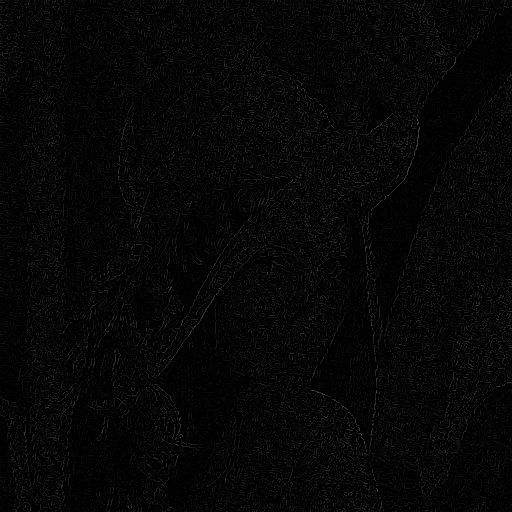
\includegraphics[width=\textwidth]{imagenesInforme/lenaNonMaximumSupressionRayleighRoberts}
	\caption{Roberts}
	\end{subfigure}
\caption{Con ruido Rayleigh multiplicativo y non-maximum supression}
\end{figure}

En el caso del ruido Rayleigh, se puede notar que su impacto es considerable. Aunque no se vé bien en estas figuras, en el caso de Roberts, la imagen también ha sido contaminada y se introducen varios bordes falsos.

\begin{figure}[H]
\centering
	\begin{subfigure}[t]{0.3\textwidth}
	\centering
	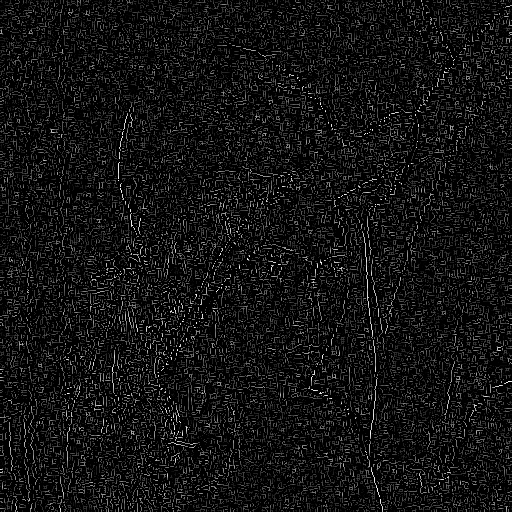
\includegraphics[width=\textwidth]{imagenesInforme/lenaNonMaximumSupressionSaltAndPepperSobel}
	\caption{Sobel}
	\end{subfigure}
	\begin{subfigure}[t]{0.3\textwidth}
	\centering
	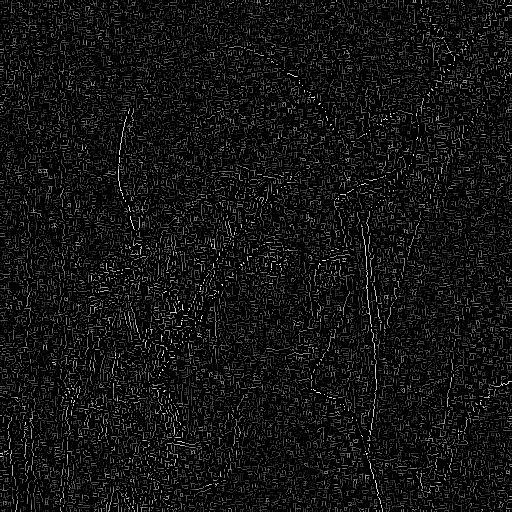
\includegraphics[width=\textwidth]{imagenesInforme/lenaNonMaximumSupressionSaltAndPepperPrewitt}
	\caption{Prewitt}
	\end{subfigure}
	\begin{subfigure}[t]{0.3\textwidth}
	\centering
	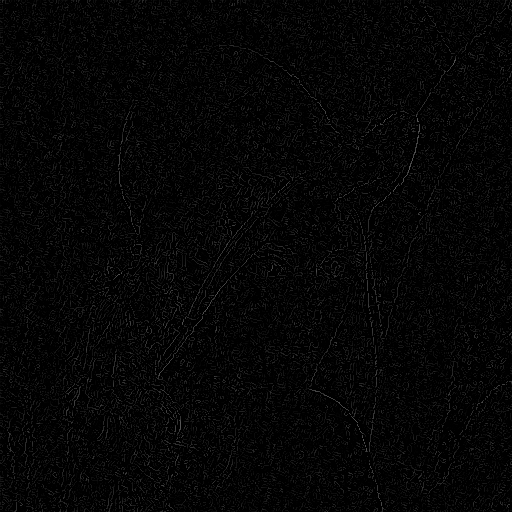
\includegraphics[width=\textwidth]{imagenesInforme/lenaNonMaximumSupressionSaltAndPepperRoberts}
	\caption{Roberts}
	\end{subfigure}
\caption{Con ruido sal y pimienta, y non-maximum supression}
\end{figure}

El ruido sal y pimienta es el que arruina más la detección de bordes. Esto es de esperarse, ya que introduce varios puntos de alto contraste (blancos y negros) en la imagen, que se reflejan en su gradiente.

\subsection*{Histéresis}

\begin{figure}[H]
\centering
	\begin{subfigure}[t]{0.3\textwidth}
	\centering
	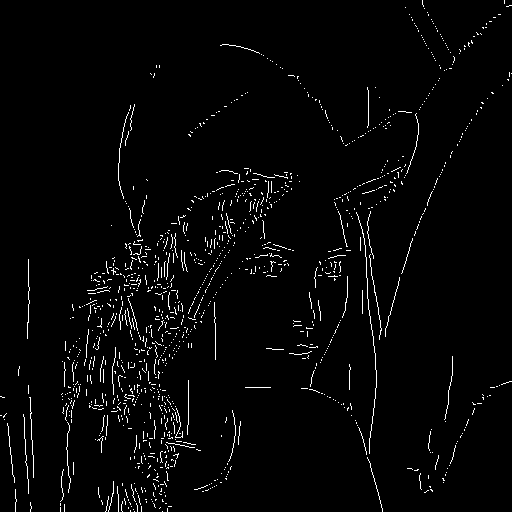
\includegraphics[width=\textwidth]{imagenesInforme/lenaHysteresisSobel}
	\caption{Sobel}
	\end{subfigure}
	\begin{subfigure}[t]{0.3\textwidth}
	\centering
	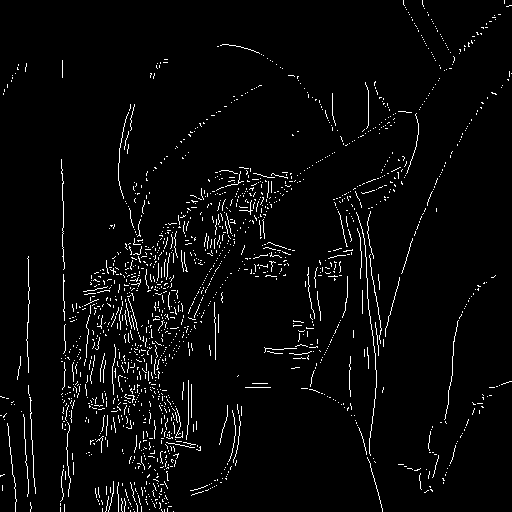
\includegraphics[width=\textwidth]{imagenesInforme/lenaHysteresisPrewitt}
	\caption{Prewitt}
	\end{subfigure}
	\begin{subfigure}[t]{0.3\textwidth}
	\centering
	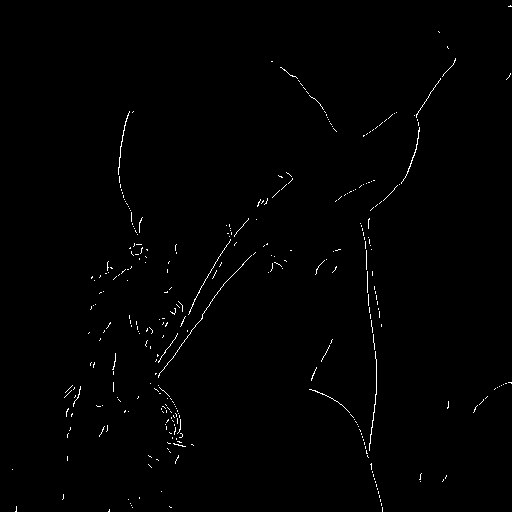
\includegraphics[width=\textwidth]{imagenesInforme/lenaHysteresisRoberts}
	\caption{Roberts}
	\end{subfigure}
\caption{Con histéresis sin ruido}
\end{figure}

Las imágenes con histéresis definen bordes y eliminan aquellos que no están en cierto umbral. Si queremos bordes bien definidos, este paso es necesario. Es también importante encontrar buenos parámetros de umbrales superior e inferior. En este caso, Roberts podría haber usado un umbral superior menor.

\begin{figure}[H]
\centering
	\begin{subfigure}[t]{0.3\textwidth}
	\centering
	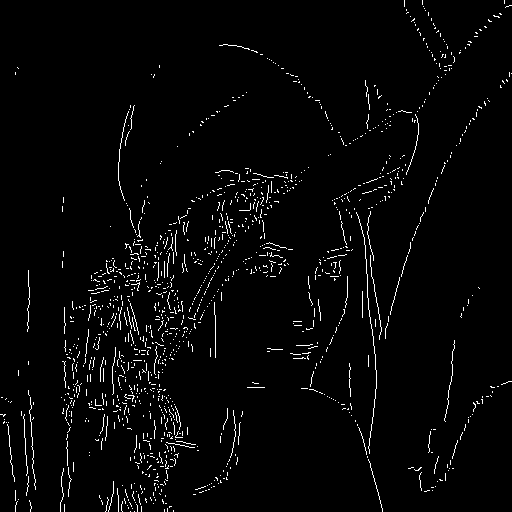
\includegraphics[width=\textwidth]{imagenesInforme/lenaHysteresisGaussianSobel}
	\caption{Sobel}
	\end{subfigure}
	\begin{subfigure}[t]{0.3\textwidth}
	\centering
	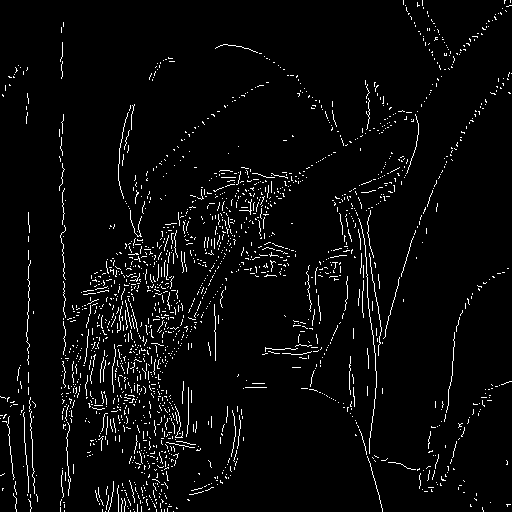
\includegraphics[width=\textwidth]{imagenesInforme/lenaHysteresisGaussianPrewitt}
	\caption{Prewitt}
	\end{subfigure}
	\begin{subfigure}[t]{0.3\textwidth}
	\centering
	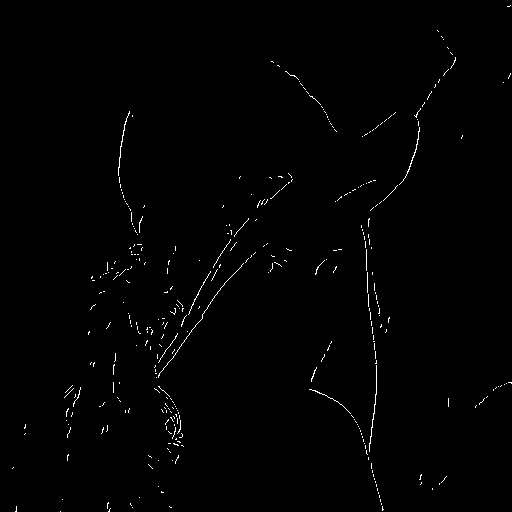
\includegraphics[width=\textwidth]{imagenesInforme/lenaHysteresisGaussianRoberts}
	\caption{Roberts}
	\end{subfigure}
\caption{Con ruido gaussiano aditivo e histéresis}
\end{figure}

Como en el caso sin histéresis, el ruido gaussiano aditivo no introduce muchos artefactos.

\begin{figure}[H]
\centering
	\begin{subfigure}[t]{0.3\textwidth}
	\centering
	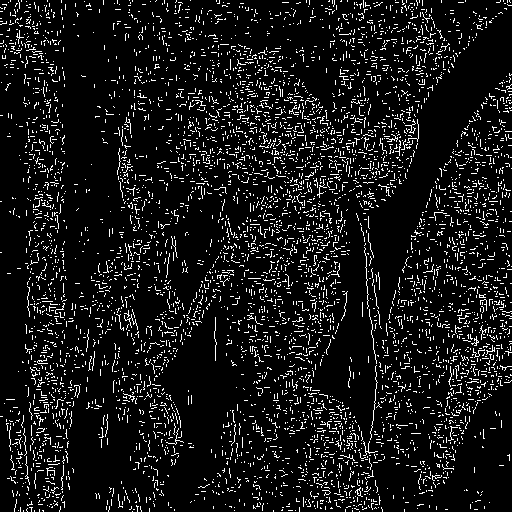
\includegraphics[width=\textwidth]{imagenesInforme/lenaHysteresisRayleighSobel}
	\caption{Sobel}
	\end{subfigure}
	\begin{subfigure}[t]{0.3\textwidth}
	\centering
	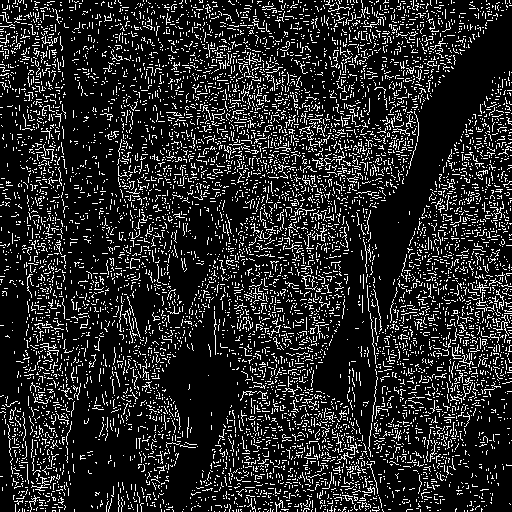
\includegraphics[width=\textwidth]{imagenesInforme/lenaHysteresisRayleighPrewitt}
	\caption{Prewitt}
	\end{subfigure}
	\begin{subfigure}[t]{0.3\textwidth}
	\centering
	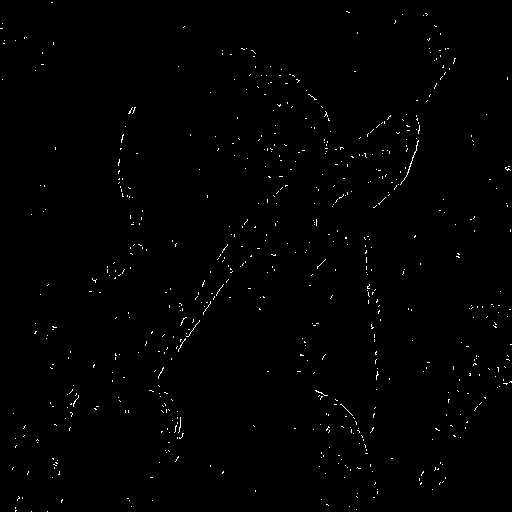
\includegraphics[width=\textwidth]{imagenesInforme/lenaHysteresisRayleighRoberts}
	\caption{Roberts}
	\end{subfigure}
\caption{Con ruido Rayleigh multiplicativo e histéresis}
\end{figure}

Contaminar la imagen con ruido Rayleigh produce muchos bordes falsos, al punto de fallar la detección, salvo en Roberts, que todavía se puede apreciar una semblanza de bordes reales, si bien cortados.

\begin{figure}[H]
\centering
	\begin{subfigure}[t]{0.3\textwidth}
	\centering
	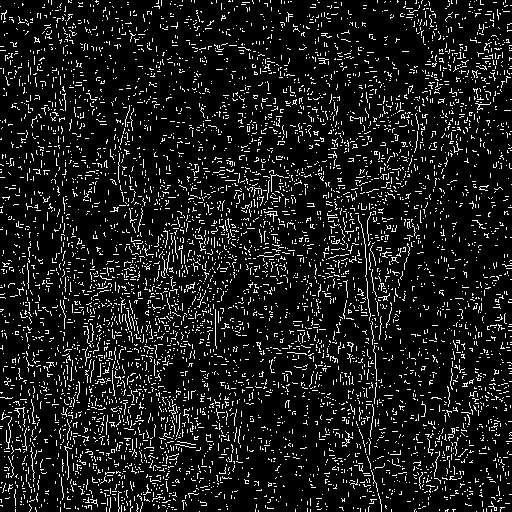
\includegraphics[width=\textwidth]{imagenesInforme/lenaHysteresisSaltAndPepperSobel}
	\caption{Sobel}
	\end{subfigure}
	\begin{subfigure}[t]{0.3\textwidth}
	\centering
	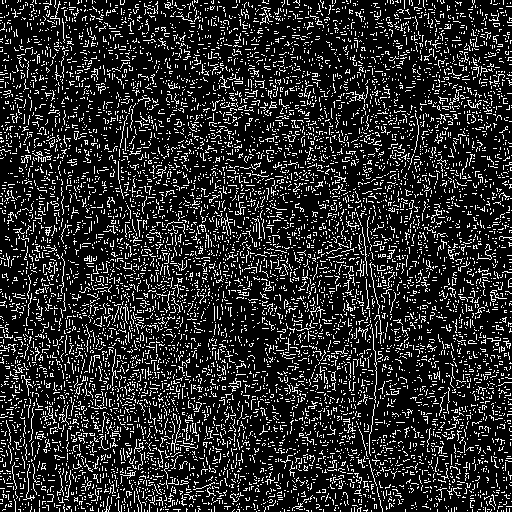
\includegraphics[width=\textwidth]{imagenesInforme/lenaHysteresisSaltAndPepperPrewitt}
	\caption{Prewitt}
	\end{subfigure}
	\begin{subfigure}[t]{0.3\textwidth}
	\centering
	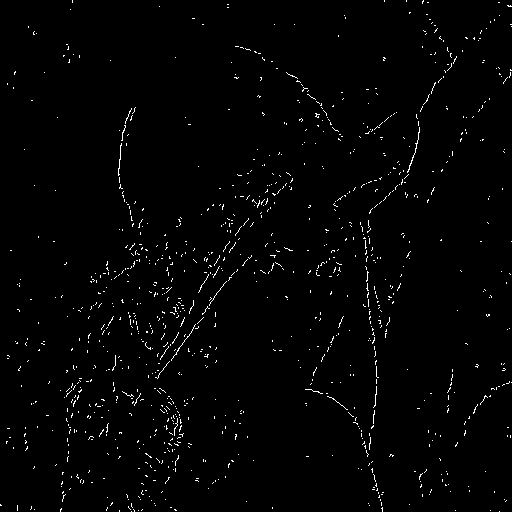
\includegraphics[width=\textwidth]{imagenesInforme/lenaHysteresisSaltAndPepperRoberts}
	\caption{Roberts}
	\end{subfigure}
\caption{Con ruido sal y pimienta, e histéresis}
\end{figure}

Salvo en Roberts otra vez, aplicar ruido impulsivo a la imagen arruina la detección de bordes. Tanto es así que en Prewitt no puede ni distinguirse la forma de la imagen original. Roberts todavía logra detectar los bordes bien sin la introducción de muchos bordes falsos.

\subsection*{Conclusiones}

Podemos observar entonces que el paso de histéresis define mejor los bordes eliminando aquellos afuera de un umbral, pero sin embargo es mucho más susceptible al ruido. Sobre todo al sal y pimienta, que arruina completamente la imagen, salvo usando Roberts como kernel.

\end{document}
